\chapter{Deep Learning Basics}
\label{ch:deep-learning-basics}

Deep learning is part of machine learning methods which learns data representations automatically. Categorized by the type of input data, learning can be supervised, semi-supervised, and unsupervised. This chapter introduces some basic concepts of deep learning. 

Convolutional Neural Networks, or CNNs, are a family of neural networks for processing non-sequential data, such as static images. Much as ordinary neural networks that are made of neurons and have learnable weights and biases, convolutional neural networks utilize certain properties of the inputs, which vastly reduce the number of parameters in the network. 

Recurrent Neural Networks, or RNNs, is a type of neural network that is specialized for processing sequential data, such as video, sentence, and audio. Different from convolutional neural networks, which accept a fixed-sized vector as input and output a fixed-sized vector, RNNs are scaleable to sequences with variable length because the recurrent transformations can be applied multiple times. RNNs have many important applications, such as image captioning, machine translations, and video classification.

\section{Convolutional Neural Network} % (fold)
Regular neural networks consist of a series of hidden layers with each layer contains a set of neurons. Neurons in each layer are independent to each other, but they have connections to all neurons in the previous layer. Thus the full-connected structure cannot be used for processing large images. For example, there would be $120,000$ weights for a single neural network with only one hidden layer  to encode images of size $200\times200\times3$.

In convolutional neural networks, neurons in a layer will only be connected to a small region of the layer before it. In other words, the hidden neurons in layer $l$ are from a subset of neurons in layer $l-1$ as shown in Figure \ref{dl:cnn}. Neurons in layer $l$ are only connected to 3 adjacent neurons in layer $l-1$. CNNs learn ``filters'' to encode the local visual patterns. In addition, each filter can be applied multiple times. In Figure \ref{dl:cnn}, weights of the same color are identical which allows the visual patterns to be detected regardless of their locations in the input images. By sharing weights, CNNs can greatly reduce the number of parameters and increase learning efficiency. Convolutional neural networks have better generalization capacity on vision problems than regular neural networks.

A typical convolutional neural network is a sequence of linear and non-linear operators. The output of the previous layer serves as the input of the next layer. A simple CNN model for classification could have the architecture as shown in Figure \ref{dl:cls}. The neural network mainly consists of four types of layers: Convolutional Layer, Pooling Layer, ReLU Layer, and Fully-Connected Layer. Some layers have parameters and others don't. Next, we will introduce these layers.


%----------------------------------------------------------------------------------
\begin{figure}
\begin{center}
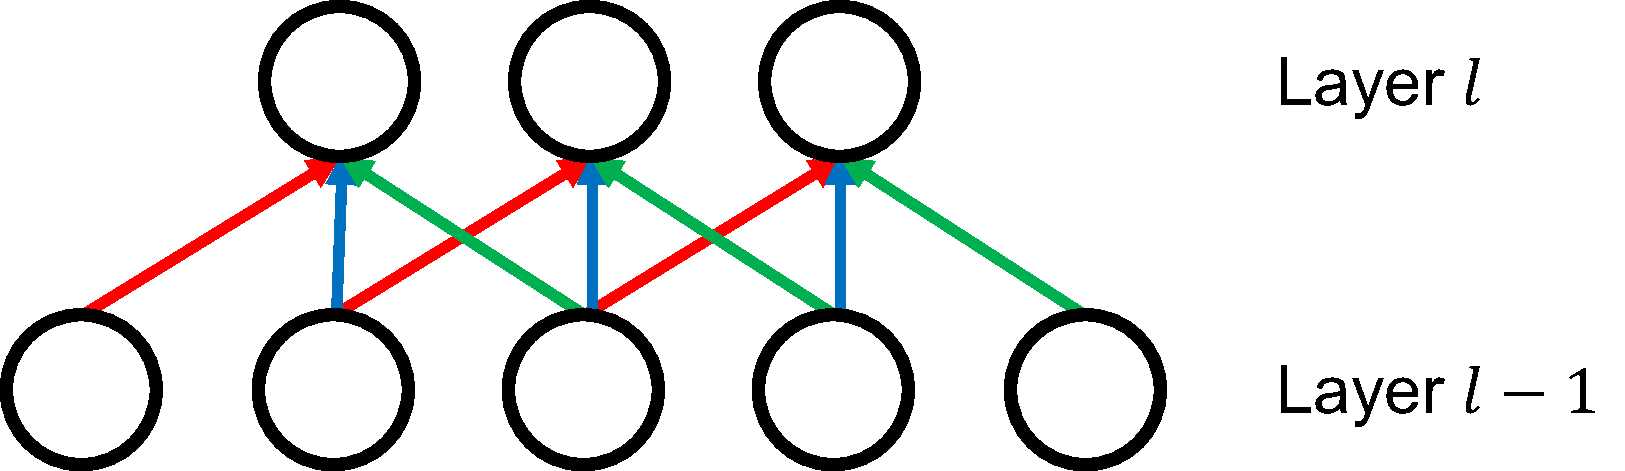
\includegraphics[width=0.7\linewidth]{figures/cnn.pdf} \ \\
\end{center}
\caption{Illustration of convolutional neural networks with shared weights.}
\label{dl:cnn}
\end{figure}
%----------------------------------------------------------------------------------


\subsection{Convolutional Layer}
Convolutional operation is the main workhorse in CNNs. The use of filters in convolutional layers greatly reduces the model size. For example, a filter on the first layer might have size $3\times 5\times 5$ (5 pixels width and height for capturing the spatially local information, and 3 because images have 3 color channels). During the forward propagation, we slide the filter across the whole image and compute the inner products of the filter weight and the input at each position. 
A general form of the convolutional operation can be written as follows:
\begin{equation}
  y(i,j) = b + \sum_{c=1}^C \sum_{p=-K}^K \sum_{q=-K}^K w(c,p,q) x(c,i+p,j+q),
\end{equation}
where $x\in\mathbb{R}^{C\times H\times W}$ is the input with spatial size $H \times W$ and $C$ channels, $w\in\mathbb{R}^{C\times (2K+1)\times (2K+1)}$ is the parameter matrix of a filter. $b\in\mathbb{R}$ is the bias. $2K+1$ is the filter size. $y\in{H\times W}$ is an output feature map. 

The filters will generate different feature maps, and thus they serve as pattern detectors to find different types of visual features such as shapes, edges, or colors in the input image.

%----------------------------------------------------------------------------------
\begin{figure}
\begin{center}
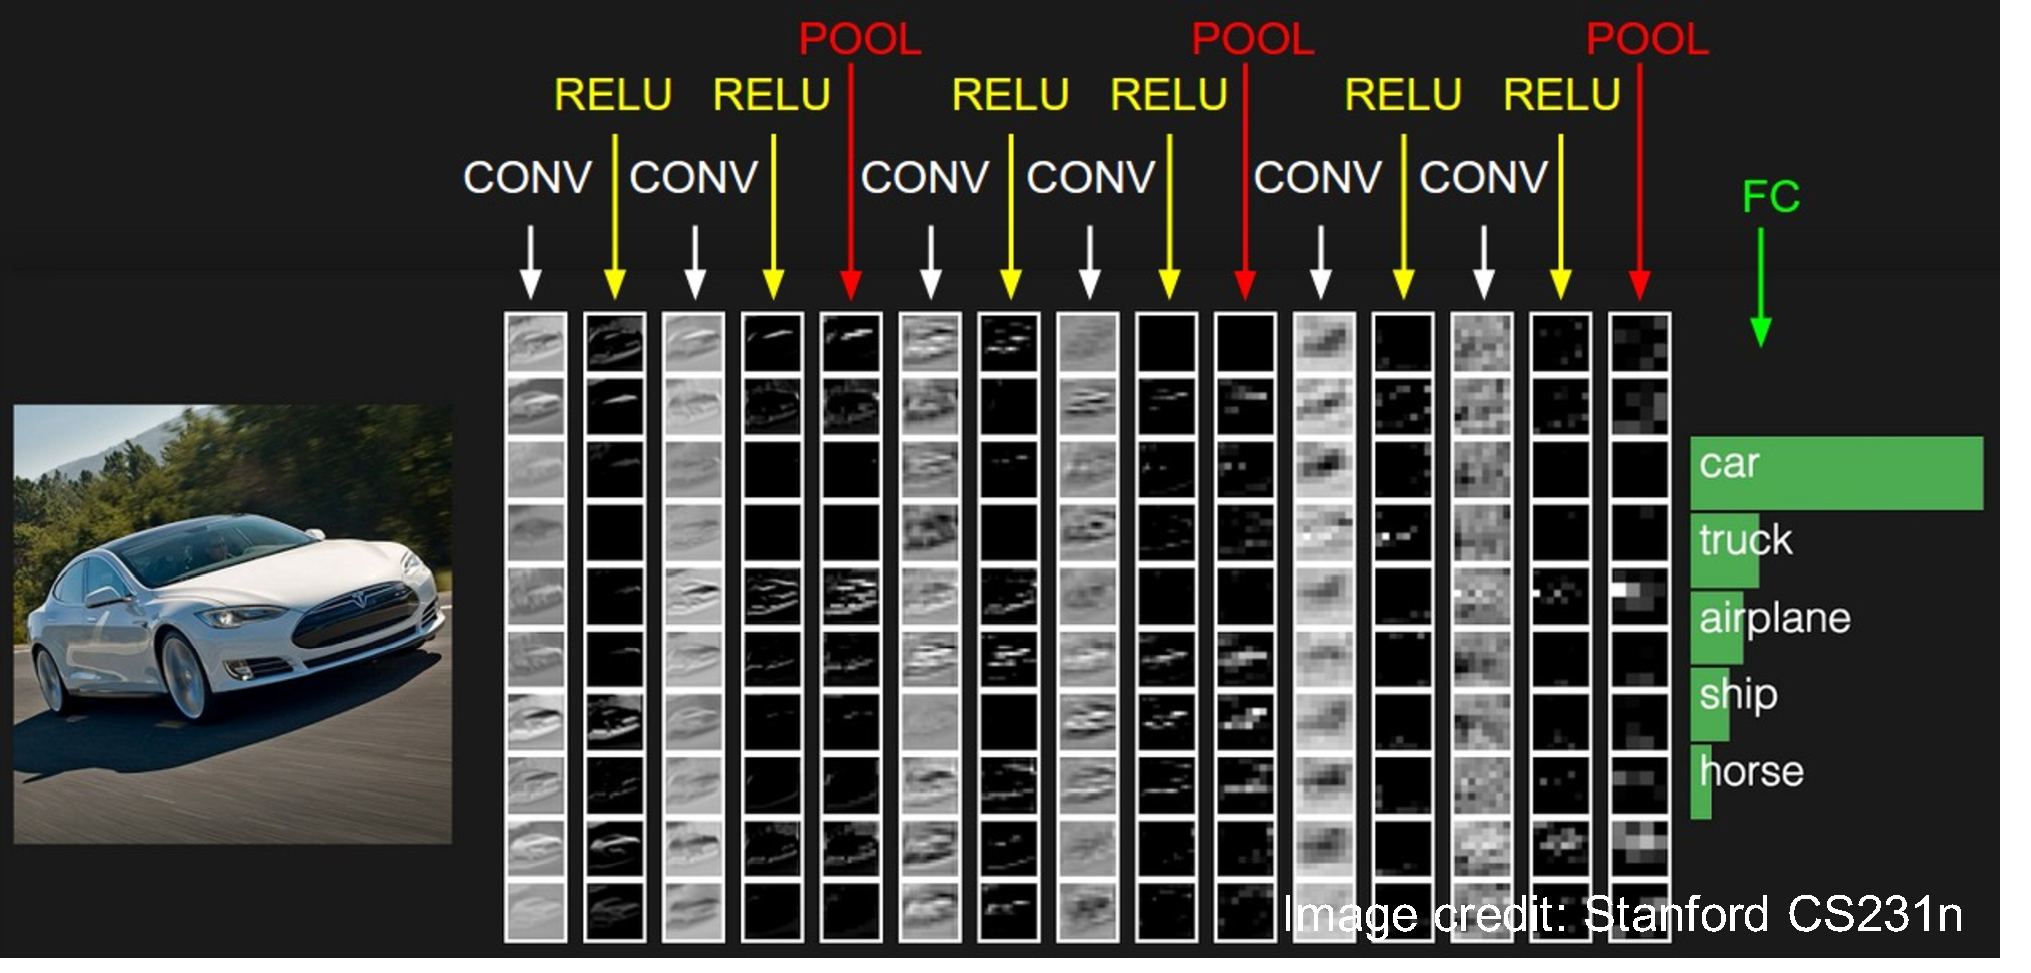
\includegraphics[width=1\linewidth]{figures/convnet.pdf} \ \\
\end{center}
\caption{An example CNN architecture for image classification. Source: Stanford CS231n}
\label{dl:cls}
\end{figure}
%----------------------------------------------------------------------------------

\subsection{Fully-Connected Layer}
Fully-connected layer is a linear mapping:
\begin{equation}
  y=Wx+b,
\end{equation}
where $x\in\mathbb{R}^d$ is the input vector,  $W\in\mathbb{R}^{m\times d}$ and $b\in\mathbb{R}^m$ are the weight matrix and bias vector respectively. Neurons in the fully-connected layer are connected to all neurons in the previous layer, and thus fully-connected layers have more parameters than convolutional layers. FC layers are often added to the end of a neural network to predict class probabilities.

\subsection{ReLU Layer and Softmax Layer}
The ReLU activation function has become popular in the past few years. It has the mathematical form:
\begin{equation}
  \mathrm{ReLU}(x) = \begin{cases}
    x & \text{when }x \ge 0,\\
    0 & \text{when }x < 0.
  \end{cases}
\end{equation}
The ReLU layer thresholds a matrix of activation at zero. It is very easy to be implemented. However, the ReLU function could cause neurons never activate on any datapoint again because of the $x<0$ part. 

Leakey ReLU modifies the ReLU function to fix the "dying ReLU" problem. The Leakey ReLU adopts a slope in the negative region:
\begin{equation}
  \mathrm{Leakey ReLU}(x) = \begin{cases}
    x & \text{when }x \ge 0,\\
    \alpha x & \text{when }x < 0,
  \end{cases}
\end{equation}
where $\alpha$ is a small constant.

Softmax is another commonly used non-linear function. It squashes the output of each item to be in $(0,1)$ and forces the sum of the output to be 1. The mathematical form is shown as follows:
\begin{equation} \label{eq:softmax}
  \mathrm{softmax}(x)_i=\frac{\exp(x_i)}{\sum_{j=1}^d \exp(x_j)}.
\end{equation}
The outputs of softmax layer equal to the categorical probability distribution and can be sent to the loss function with target label to compute losses. 

\subsection{Pooling Layer}
Pooling layer is another important operator. It is commonly inserted between two convolutional layers for reducing the parameter size. Pooling is a form of down-sampling along the spatial dimensions. The most common form is the max pooling with filters of size $2\times 2$. 

Max-pooling divides the input feature map into a set of non-overlapping grids and outputs the maximum value in each grid. The depth dimension remains unchanged, but the spatial size would decrease following the formulation: $H_o = (H-F)/F+1$, $W_o = (W-F)/F+1$. $H$ and $W$ are the input height and width, $F$ is the filter size, and $S$ is the stride of down-sampling along both the width and height.

%----------------------------------------------------------------------------------
\begin{figure}
\begin{center}
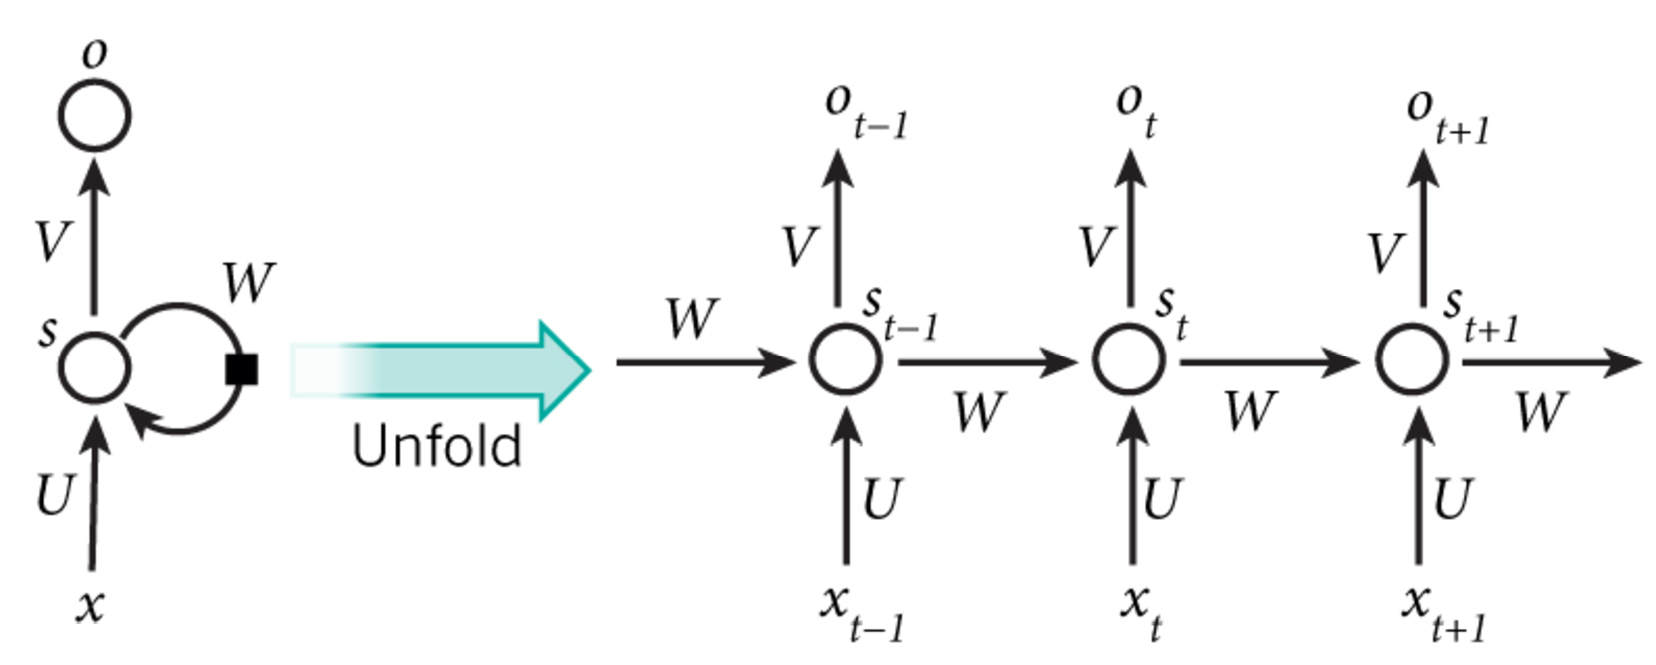
\includegraphics[width=0.9\linewidth]{figures/rnn.pdf} \ \\
\end{center}
\caption{A recurrent neural network and the unfolding form. Source: Nature}
\label{dl:rnn}
\end{figure}
%----------------------------------------------------------------------------------

\section{Recurrent Neural Network}
The idea of RNNs is to utilize sequential information. A typical RNN model is shown in Figure \ref{dl:rnn}. The RNN is unrolled into a full network. In the forward propagation, we send the sequential data to the neural network one by one and get an output at each time step (this is not necessary, for some specific tasks, we may only care about the final output). The RNN shares parameters across all steps to reduce the parameter size.

Long Short-Term Memory (LSTM) and Gated Recurrent Unit (GRU) are the most commonly used RNNs. LSTMs and GRUs have the same architecture as RNNs, but they use different ways to compute the hidden state $s_t$. $x_t$ and $o_t$ are the input and output at time step $t$ in Figure \ref{dl:rnn}. $U, W, V$ are transformation matrices. Next, we will take the machine translation as an example to introduce LSTM and GRU models.

\subsection{Long Short-Term Memory}
RNN models encode sequential data and utilize previous information to the present task. However, RNNs tend to focus on the most recent inputs and forget the beginning ones. When the input sequence is too long, the gap between the relevant information and point where it is needed becomes very large which makes the RNNs cannot connect that information.

Long short-term memory networks are designed by Hochreiter \etal~\cite{hochreiter1997long} to avoid the long-term dependency problem. There are three gates and one memory cell in LSTMs. The gates control the flow direction of information while the memory cell preserves knowledge of previous steps. At each word, the LSTMs update the memory cell $c_t$ and output a hidden state $h_t$ in the following way:
\begin{align}
i_t &= \sigma{(W_{xi} x_t + W_{hi} h_{t-1} + b_i)}, \nonumber \\
f_t &= \sigma{(W_{xf} x_t + W_{hf} h_{t-1} + b_f)}, \nonumber \\
o_t &= \sigma{(W_{xo} x_t + W_{ho} h_{t-1} + b_o)}, \\
c_t &= f_t \odot c_{t-1} + i_t \odot h{(W_{xc} x_t + W_{hc} h_{t-1} + b_c)}, \nonumber\\
s_t &= o_t \odot h{(c_t)}, \nonumber
\end{align}
where $\odot$ represents the element-wise multiplication, $W$ and $b$ are parameters to be learned, $sigma$ and $h$ are the sigmoid function and tanh function respectively.
The forget gate $f$ is a sigmoid function, which looks at the hidden state of the last step $h_{t-1}$ and the input word $x_t$, and outputs a scalar to indicate which value to be thrown away from the cell state. The input gate $i$ and output gate $o$ decide which information to be updated and output respectively. $c$ is a function of the old subjects and the new input.

\subsection{Gated Recurrent Unit}
GRU model is first introduced by Kyunghyun \etal~\cite{cho2014learning}. It has a simpler structure and fewer parameters than LSTM. The implementation is shown below:
\begin{align}
z_t &= \sigma{(W_{xz} x_t + W_{hz} h_{t-1} + b_z)}, \nonumber \\
r_t &= \sigma{(W_{xr} x_t + W_{hr} h_{t-1} + b_r)}, \nonumber \\
h_t &= h(W_{xh} x_t  + W_{hh} (r_t \odot s_{t-1}) + b_h), \nonumber \\
s_t &= (1-z_t) \odot s_{t-1}  + z_t \odot h_t, \nonumber
\end{align}

A GRU has two gates, a reset gate $r$ and an update gate $z$. The reset gate decides how to combine the new and old information. The update gate determines which value to be kept.
Different from LSTMs, which have three gates and an internal memory cell $c_t$, GRUs don't have the output gate. The reset gate is applied directly to the previous hidden state. Because of the fewer parameters, GRUs need less time and data to generalize when training.


\section{Deep Learning Applications} % (fold)
\subsection{Image Classification}
Deep convolutional neural networks have led to great success for large-scale image classification. AlexNet~\cite{krizhevsky2012imagenet} roses the interest in CNNs. It is considered to be the break-through method when winning the ImageNet challenge of 2012. The network consists of 5 convolutional layers, 3 fully-connected layers, and some dropout layers and max-pooling layers. It also contains data augmentation and ReLU non-linear activation functions. VGG Net\cite{simonyan2014very} replaces the $7\times 7$ filters in AlexNet with $3\times 3$ filters. The intuition is that 2 consecutive $3\times 3$ filters and a $5\times 5$ filter have the same receptive field, and thus 3 consecutive $3\times 3$ filters give a receptive field of a $7\times 7$ filter. The introduction of smaller filters reduce the number of parameters and the deep models can be designed deeper. 

GoogLeNet~\cite{szegedy2015going} has several inception modules and eliminates all fully-connected layers which save lots of parameters. Microsoft Resnet~\cite{he2016deep} wins the 2015 ImageNet challenge. The Residual block is represented as follows:
\begin{equation}
  y = f_\theta(x) + x,
\end{equation}
He \etal show the model introduces neither extra parameter nor computation complexity, and can be designed very deep.

\subsection{Object Detection}
Object detection aims at identifying the location of objects in an image. Early methods~\cite{girshick2014rich} generate regions of interest or region proposals and send them to CNN models to learn feature representations. In \cite{girshick2014rich}, Girshick \etal propose the Fast R-CNN which significantly improves the training and testing speed and accuracy. Instead of extracting features of each candidate bounding box, they forward the image only once and the features of each bounding box are generated by a RoI pooling layer. However, the detection accuracy of Fast R-CNN depends on the performance of the region proposal module. 

Faster R-CNN~\cite{ren2015faster} combines the proposal detection and Fast R-CNN in a single deep neural network. They introduce a novel Region Proposal Network that shares convolutional layers with down-stream detection networks. The RPN predicts object bounds and objectness scores at each position simultaneously which enables nearly cost-free region proposals. Faster R-CNN realizes the real-time object detection.

\subsection{Generative Adversarial Networks}
Generative adversarial networks (GANs) are deep neural networks comprised of a generator (G) and a discriminator (D). The generator takes random inputs and generates new data instances to fool the discriminator. The discriminator tries to classify whether the input data belonging to the actual training dataset or not. The generator and discriminator play the following minimax game:
\begin{equation}
  \min\limits_{G} \max\limits_{D} V(D, G) = \mathbb{E}_{x\sim p_{data}}[log D(x)] + \mathbb{E}_{x\sim p_{z}(z)}[log(1-D(G(z)))],
\end{equation}

DCGAN~\cite{radford2015unsupervised} introduces deep convolutional neural networks to generative adversarial models and shows that the deep generative networks can learn good representations of images. Wasserstein GAN~\cite{arjovsky2017wasserstein} provides comprehensive theoretical analysis of GAN models.